\chapter{Results}\label{cha:results}

This chapter presents the results from the experiments conducted to evaluate the performance of the unsupervised learning methods investigated in this thesis. The chapter is structured into three sections with results from the depth and ego motion prediction, keypoint prediction and consensus maximization respectively. The metrics used to evaluate the networks are detailed in the evaluation metrics section \ref{sec:metrics} in the method chapter.

\section{Depth and ego motion}

For the depth and ego motion prediction networks 12 different configurations (Table \ref{table:configurations}) were trained and evaluated in 16 experiments (Table \ref{table:experiments}). The configurations and experiments are named C1 trough C12 and E1 to E16 respectively. A configuration is a particular combination of options (Table \ref{table:cli}), such as dataset, network architecture and loss function terms used during training. Each experiment measures the performance, using the metrics in section \ref{sec:depthmetrics}, of a configuration on a particular testing dataset. In some experiments, the testing dataset will differ from the training dataset, for example a network can be trained on Kitti but evaluated on Lyft.

\begin{table}[H]
\centering
\begin{tabular}{|l|c|c||c|c||c|c||c|c|c|c|}
\hline
C & Net & DS & Edge & Norm & Expl & Stat & SSIM & Comb & US \\
\hline
1 & SL & K &  &  &  &  &  & avg &  \\
\hline
2 & SL & K &  &  & $ \times $ &  &  & avg &  \\
\hline
3 & SL & K &  &  &  & $ \times $ &  & avg &  \\
\hline
4 & SL & K & $ \times $ &  &  & $ \times $ &  & avg &  \\
\hline
5 & SL & K & $ \times $ &  &  & $ \times $ & $ \times $ & min &  \\
\hline
6 & SL & K & $ \times $ & $ \times $ &  & $ \times $ & $ \times $ & min &  \\
\hline
7 & SL & K & $ \times $ & $ \times $ &  & $ \times $ & $ \times $ & min & $ \times $ \\
\hline
8 & SL & L & $ \times $ & $ \times $ &  & $ \times $ & $ \times $ & min & $ \times $ \\
\hline
9 & M2 & K &  &  &  & $ \times $ &  & avg &  \\
\hline
10 & M2 & K & $ \times $ & $ \times $ &  & $ \times $ & $ \times $ & min &  \\
\hline
11 & M2 & K & $ \times $ & $ \times $ &  & $ \times $ & $ \times $ & min & $ \times $ \\
\hline
12 & M2 & L & $ \times $ & $ \times $ &  & $ \times $ & $ \times $ & min & $ \times $ \\
\hline
\end{tabular}
\caption{All configurations of the depth and ego motion network that were evaluated. The C column identifies the specific configuration. The Net column shows which architecture was used, either SL for SfmLearner or M2 for Monodepth2. The DS column shows which dataset was used during training, either K for Kitti or L for Lyft. The Edge column indicates if the edge aware smoothing loss term $\mathcal{L}_{\mathrm{edge}}$ was used. The Norm column indicates if depth map normalization was used. The Expl column indicates if an explainability mask was used. The Stat column indicates if a mask to remove stationary pixels from the loss was used. The SSIM column indicates if $\mathcal{L}_{\mathrm{ps}}$ was used, otherwise just $\mathcal{L}_{p}$. The Comb column shows which methods was used to combine the loss terms from the two source images, either the average or the minimum loss across frames. The US column indicates that up-scaling of the depth maps in the pyramid was used, otherwise the target frame was down-scaled to match the size of the smaller depth maps in the pyramid.}
\label{table:configurations}
\end{table}


\begin{table}[H]
\centering
{\setlength{\tabcolsep}{0.4em}
\begin{tabular}{|r|r|c||l|l|l|l||l|l|l||l|}
\hline
E & C & DS & AbsRel & SqRel & RMSE & RMSLE & $1.25$ & $1.25^2$ & $1.25^3$ & Ego \\
\hline
1 & 1 & K & 0.174 & 1.405 & 4.829 & 0.249 & 0.784 & 0.920 & 0.964 & 0.024 \\
\hline
2 & 2 & K & 0.179 & 1.686 & 4.880 & 0.252 & 0.782 & 0.919 & 0.961 & 0.021 \\
\hline
3 & 3 & K & 0.140 & 0.793 & 4.549 & 0.217 & 0.818 & 0.939 & 0.976 & 0.020 \\
\hline
4 & 4 & K & 0.143 & 0.819 & 4.708 & 0.222 & 0.810 & 0.937 & 0.975 & 0.022 \\
\hline
5 & 5 & K & 0.133 & 0.727 & 4.305 & 0.204 & 0.843 & 0.950 & 0.979 & 0.023 \\
\hline
6 & 6 & K & 0.137 & 0.797 & 4.282 & 0.208 & 0.837 & 0.948 & 0.977 & 0.024 \\
\hline
\hline
7 & 7 & K & 0.135 & 0.778 & 4.248 & 0.208 & 0.841 & 0.948 & 0.997 & 0.020 \\
\hline
8 & 7 & L & 0.340 & 7.811 & 23.071 & 0.447 & 0.457 & 0.734 & 0.868 & 0.043 \\
\hline
9 & 8 & K & 0.512 & 5.185 & 10.757 & 0.611 & 0.305 & 0.549 & 0.732 & 0.495 \\
\hline
10 & 8 & L & 0.739 & 20.236 & 31.859 & 0.773 & 0.240 & 0.434 & 0.587 & 1.324 \\
\hline
\hline
11 & 9 & K & \textbf{0.125} & \textbf{0.697} & 4.298 & 0.203 & 0.845 & 0.948 & 0.979 & 0.021 \\
\hline
12 & 10 & K & 0.126 & 0.714 & 4.018 & \textbf{0.194} & \textbf{0.860} & \textbf{0.958} & \textbf{0.982} & \textbf{0.019} \\
\hline
\hline
13 & 11 & K & 0.132 & 0.769 & \textbf{3.966} & 0.196 & 0.859 & 0.957 & 0.981 & \textbf{0.019} \\
\hline
14 & 11 & L & 0.304 & 7.019 & 21.907 & 0.414 & 0.518 & 0.775 & 0.886 & 0.042 \\
\hline
\hline
15 & 12 & K & 0.322 & 3.177 & 7.179 & 0.378 & 0.549 & 0.797 & 0.906 & 0.036 \\
\hline
16 & 12 & L & 0.303 & 8.051 & 19.312 & 0.385 & 0.637 & 0.827 & 0.906 & 0.059 \\
\hline
\end{tabular}}
\caption{All the experiments measuring the performance of the different configurations in Table \ref{table:configurations}. The best result for each column is written in bold numerals. The E column identifies a specific experiment. The C column shows which configuration was used. The DS column shows which dataset was used during testing, K for Kitti and L for Lyft. The dataset used during testing differs from the one used during training in some experiments. The AbsRel, SqRel, RMSE and RMSLE columns are the depth error metrics described in section \ref{sec:depthmetrics}, smaller is better. The $1.25$, $1.25^2$ and $1.25^3$ columns are the depth accuracy metrics described in section \ref{sec:depthmetrics}, larger is better. The Ego column is the camera ego motion error metric described in section \ref{sec:egometric}.}
\label{table:experiments}
\end{table}

To verify the quality of the predictions visually, the depth map can be rendered using two different methods. Either as tinted depth map where black pixels are further away than yellow pixels (Figure \ref{fig:depthmapskitty}), or as a 3D point cloud where each point is colored by the input image (Figure \ref{fig:3drender}).

\begin{figure}[H]
	\centering
	\begin{minipage}{.5\textwidth}
		\centering
		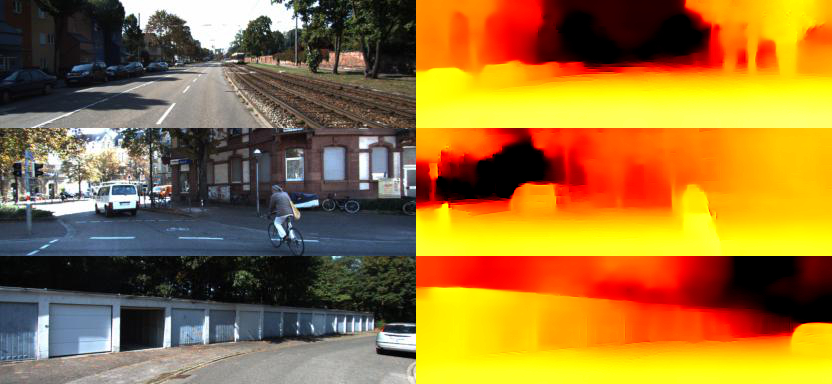
\includegraphics[width=1.0\linewidth]{depthmaps}
		\captionof{figure}{Three depth maps from experiment E13, which is the Monodepth2 architecture with all options enabled, trained and evaluated on the Kitty dataset.}
		\label{fig:depthmapskitty}
	\end{minipage}%
	\begin{minipage}{.5\textwidth}
		\centering
		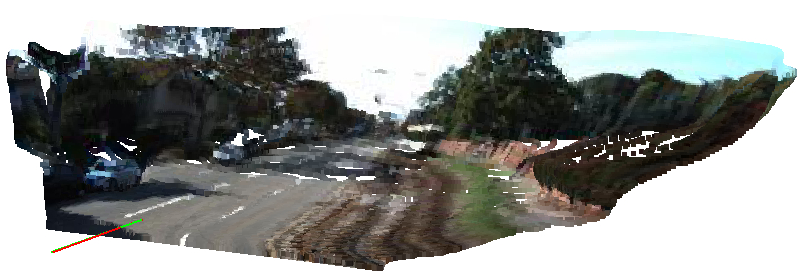
\includegraphics[width=1.0\linewidth]{3drender}
		\captionof{figure}{One depth map from experiment E13 rendered as a colorized point cloud.}
		\label{fig:3drender}
	\end{minipage}
\end{figure}

The point cloud of a particular image can be rendered from different perspectives by a virtual camera (Figure \ref{fig:3dseq}). The virtual camera can be used to render a birds eye view of the 3D path built using the incremental ego motion predictions in a sequence (Figure \ref{fig:movement}).

\begin{figure}[H]
	\centering
	\begin{minipage}{.5\textwidth}
		\centering
		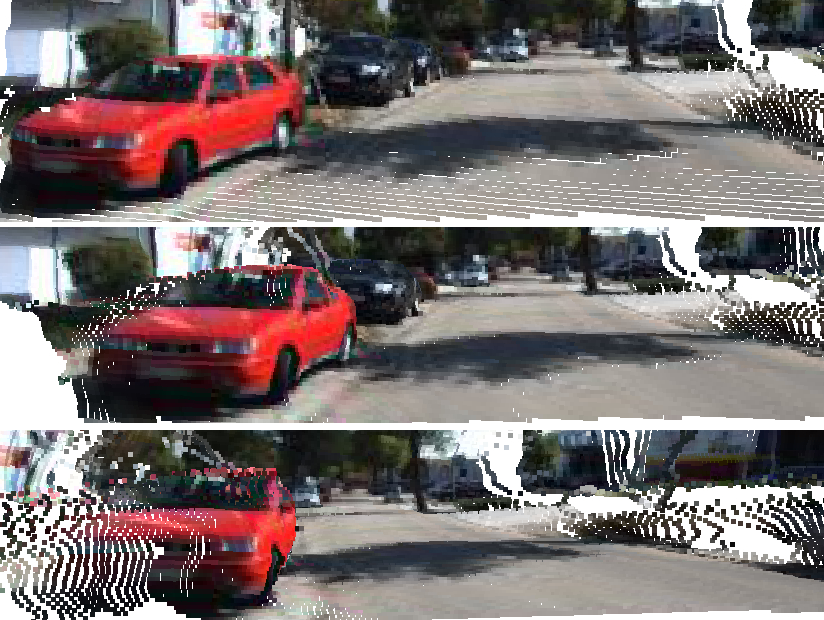
\includegraphics[width=1.0\linewidth]{3dseq}
		\captionof{figure}{A single depth map from experiment E13 rendered from 3 different angles as a colorized point cloud.}
		\label{fig:3dseq}
	\end{minipage}%
	\begin{minipage}{.5\textwidth}
		\centering
		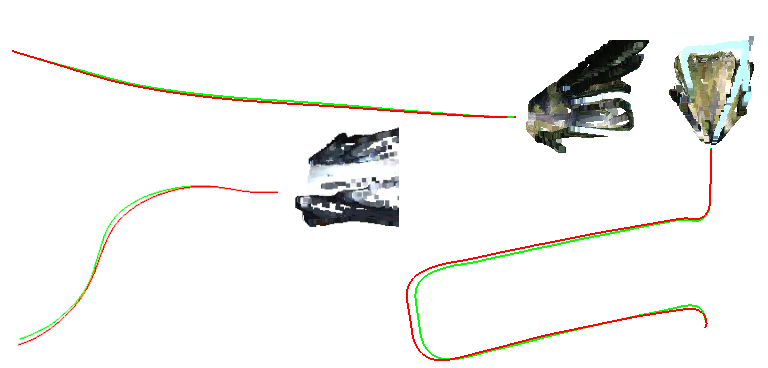
\includegraphics[width=1.0\linewidth]{motion2}
		\captionof{figure}{Camera movement in three different image sequences from experiment E13. The green lines are the ground truth and the red lines are the predicted camera trajectories.}
		\label{fig:movement}
	\end{minipage}
\end{figure}

Comparing E1 and E2, we see that the explainability mask improves the accuracy ever so slightly but the depth error is actually worse. When the stationary pixel mask is used instead in E3, the error metrics are significantly better than in both E1 and E2, the accuracy is comparable but slightly worse. The results correspond to what can be seen visually in Figure \ref{fig:e1e2e3}.

In experiment E4 the edge aware depth smoothness term is added, interestingly the performance metric does not show an improvement. But looking at one of the depth maps (Figure \ref{fig:E4}) it visually looks significantly more sharp and well defined. Probably the depth error moves to other parts of the image when the edge aware depth smoothness term is enabled.

In experiment E5 we use SSIM for the photometric reconstruction error, and also combine the loss from $\textbf{I}_{t-1}$ and $\textbf{I}_{t+1}$ using the $\min()$ function per pixel. All metrics show an improvement.

In E6 we add depth map normalization and in E7 we add upscaling, neither show any significant changes in the metrics.

In E8 we test configuration C7 on the Lyft dataset, though it was trained on Kitti. As expected, the results are worse when evaluated on a completely different dataset than the model was trained on.

In experiment E9 and E10 configuration C8 trained on Lyft is evaluated on Kitty and Lyft respectively. Very surprisingly the model performs better on Kitti even though it was trained on Lyft.

From experiment E11 and onwards the SfMLearner architecture is replaced by the Monodepth2 architecture. Both E11 and E12 shows great performance, even though E11 has a configuration which is much more bare bones than E12. This suggests that the network architecture plays a big part in the overall performance.

In E13 and E14 we again see that a network trained on Kitti performs better when evaluated on Kitti compared to Lyft, as expected. In E15 and E16 we see a network trained on Lyft that has a lower error on Kitti, but higher accuracy on Lyft.

From the results it appears that the quality of depth prediction has a pretty low impact on the performance of the ego motion estimation. The depth and ego motion is predicted by different networks. But the loss function is dependent on both depth and ego motion predictions. It is not possible to learn only depth or only ego motion separately in this system, so they are in a way coupled. But the networks are separate and the performance of the depth network does not seem to have a big impact on the performance of the ego motion network.

The effect of using either a explainability mask or stationary pixel mask can be seen in Figure \ref{fig:e1e2e3}.

\begin{figure}[H]
	\centering
	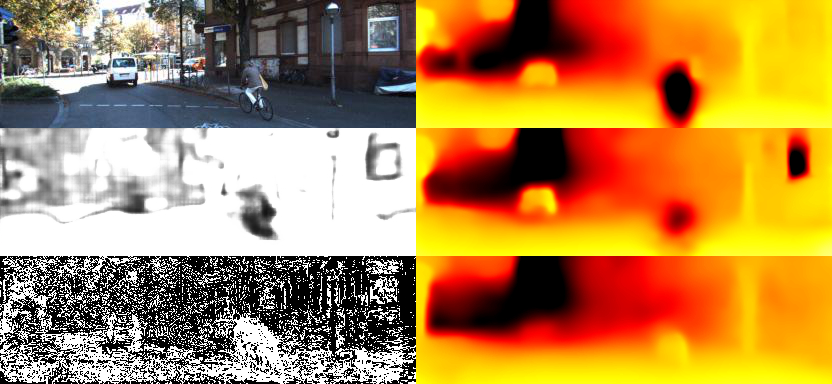
\includegraphics[width=0.8\textwidth]{E1-E2-E3}
	\caption{The top row is from experiment E1, the second row is from E2 with the explainability maps shown to the left, and the last row is from E3 with the stationary pixel map shown to the left. In the top depth map, the depth prediction for the biker is incorrect. Because the biker is stationary with respect to the camera, the disparity of the pixels across the subsequent frames becomes 0 and the depth goes to infinity. Training using an explain-ability mask seems to improve the depth prediction for the biker, and using a stationary pixels mask improves the depth even more.}
	\label{fig:e1e2e3}
\end{figure}

\begin{figure}[H]
	\centering
	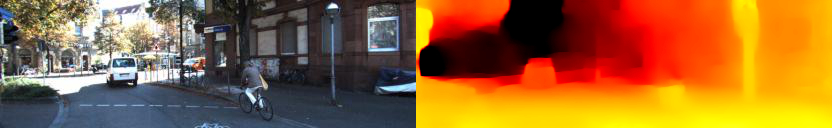
\includegraphics[width=0.8\textwidth]{E4}
	\caption{A depth map taken from experiment E4 where the edge aware smoothness loss is used.}
	\label{fig:E4}
\end{figure}

\begin{figure}[H]
	\centering
	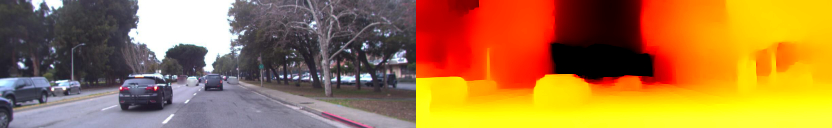
\includegraphics[width=0.8\textwidth]{E14}
	\caption{Depth map from experiment E14, where the model was trained on Kitti and evaluated on Lyft. As can be seen in the image the performance is still quite good.}
	\label{fig:E14}
\end{figure}

\begin{figure}[H]
	\centering
	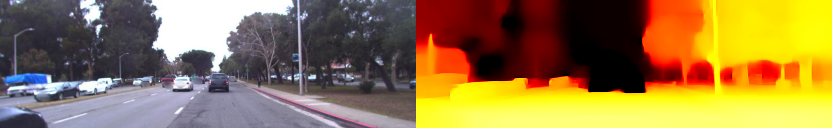
\includegraphics[width=0.8\textwidth]{E16}
	\caption{Depth map from experiment E15 where the model was trained on Lyft and also evaluated on Lyft.}
	\label{fig:E16}
\end{figure}

\iffalse
\begin{figure}[H]
	\centering
	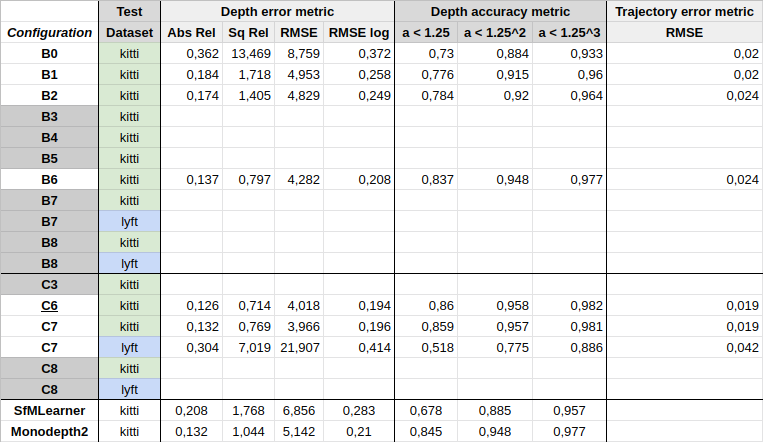
\includegraphics[width=1.0\textwidth]{evaluation}
	\caption{Evaluation metrics when testing the configurations on the testing split of the datasets}
	\label{fig:evaluation}
\end{figure}

\begin{figure}[H]
	\centering
	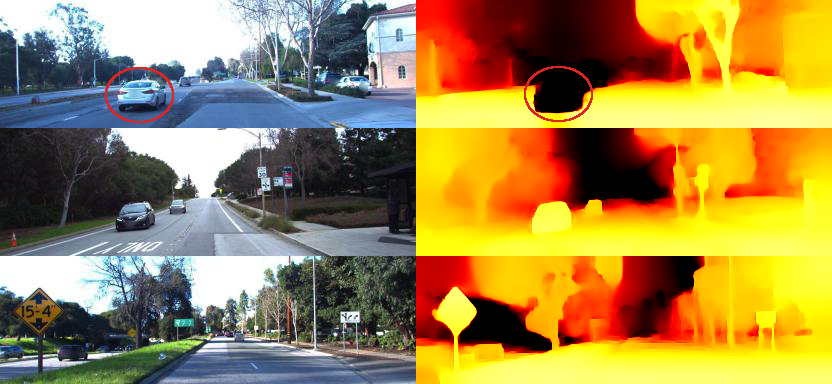
\includegraphics[width=1.0\textwidth]{depthmapslyft}
	\caption{Examples from the Lyft dataset}
	\label{fig:depthmaplyft}
\end{figure}
\fi


\section{Keypoint detection}

The keypoint predicting network was evaluated and compared with the ORB detector in OpenCV using the metrics described in section \ref{sec:keypointmetrics}. An example of the output of the keypoint prediction network can be seen in Figure \ref{fig:point1}.

\begin{figure}[H]
	\centering
	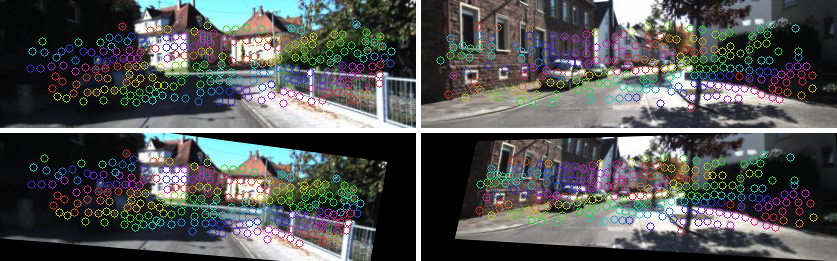
\includegraphics[width=1.0\textwidth]{point1}
	\caption{Results from the keypoint prediction network. The top row are the original input images fed to branch A, and below are the transformed images fed to branch B. Circles that are the same color have matching descriptors.}
	\label{fig:point1}
\end{figure}

\begin{table}[H]
\centering
\begin{tabular}{|l|l|l|l|l|}
\hline
Method & RS $\uparrow$ & LE $\downarrow$ & MS $\uparrow$ & MR $\uparrow$ \\
\hline
UnsuperPoint & 0.796 & \textbf{0.666} & \textbf{0.488} & \textbf{0.834} \\
ORB & \textbf{0.841} & 0.764 & 0.302 & 0.564 \\
\hline
\end{tabular}
\caption{Comparison between the keypoint predicting network and ORB detector in OpenCV. The table shows the repeatability score, localization error, matching score and matching ratio.}
\label{table:pointsbenchmark}
\end{table}

As can be seen in Table \ref{table:pointsbenchmark} the repeatability score is better for the ORB detector. This means that the ORB detector is picking points in different frames that are likely to represent the same physical feature in the world. On the other hand the keypoint network trained in this thesis has a lower localization error. The matching score and matching ratio is also better for the keypoint network, which suggests that the descriptors are better than its ORB counterpart.

\section{Consensus maximization}
The consensus maximization network was evaluated and compared with the \textit{findHomography()} function in OpenCV using the metrics described in section \ref{sec:consensusmetrics}. An example the results from the consensus maximization network can be seen in Figure \ref{fig:kittihomo}.

\begin{figure}[H]
	\centering
	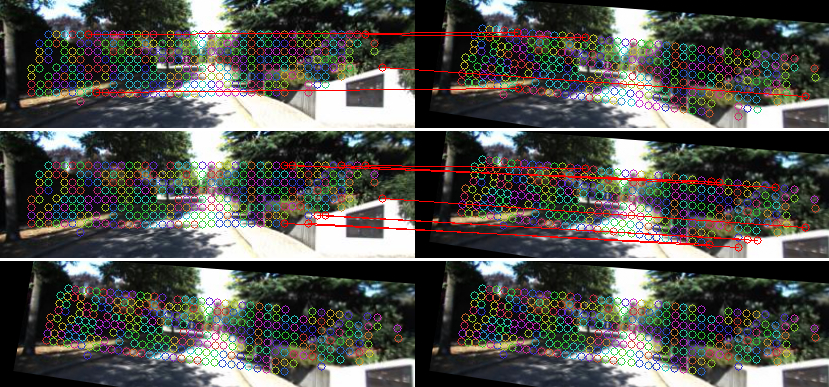
\includegraphics[width=0.9\textwidth]{kittihomo}
	\caption{Outlier prediction on homographic adaptation dataset with images from Kitti. First row shows the outliers found by OpenCV findHomography() marked in red. Second row shows the outliers found by the consensus network marked in red. In the third row the image on the left is is transformed by the homography predicted by the consensus network, and the image to the right is the image transformed by the ground truth homography.}
	\label{fig:kittihomo}
\end{figure}

\begin{table}[H]
	\centering
	\begin{tabular}{|l|l|l|l|}
		\hline
		Method & HE (std) $\downarrow$ & Best $80\%$ HE (std) $\downarrow$ \\
		\hline
		ConsensusNet & 3.97 (22.27) & 1.74 (0.82) \\
		RANSAC & 0.61 (0.45) & 0.45 (0.12) \\
		\hline
	\end{tabular}
	\caption{Comparison between the consensus maximization network and findHomography() function of OpenCV which uses the RANSAC algorithm.}
	\label{table:consensusbenchmark}
\end{table}

As can be seen in Table \ref{table:consensusbenchmark} the homography error (HE section \ref{sec:consensusmetrics}) is larger for the consensus network compared to using RANSAC. The standard deviation is very high, which suggests that the average error contains large outliers. Filtering out the best 80\% of the testing samples, we see that the standard deviation of the average homography error drops significantly. Even though the homography error is still worse than compared with RANSAC, it is not far off.

\begin{table}[H]
\centering
\begin{tabular}{l|l|c|c|c}
	\multicolumn{2}{c}{}&\multicolumn{2}{c}{Predicted}&\\
	\cline{3-4}
	\multicolumn{2}{c|}{}&Inlier&Outlier&\multicolumn{1}{c}{Total}\\
	\cline{2-4}
	\multirow{2}{*}{Actual}& Inlier & $0.964$ & $0.036$ & $\mathrm{TP}+\mathrm{FN}=1$\\
	\cline{2-4}
	& Outlier & $0.002$ & $0.998$ & $\mathrm{FP}+\mathrm{TN}=1$\\
	\cline{2-4}
	\multicolumn{1}{c}{} & \multicolumn{1}{c}{Total} & \multicolumn{1}{c}{$\mathrm{TP}+\mathrm{FP}=0.966$} & \multicolumn{    1}{c}{$\mathrm{FN}+\mathrm{TN}=1.034$} & \multicolumn{1}{c}{$2$}\\
\end{tabular}
	\caption{Confusion matrix for inlier/outlier prediction using ConsensusNet.}
	\label{table:consensusnetconfusion}
\end{table}


\begin{table}[H]
	\centering
	\begin{tabular}{l|l|c|c|c}
		\multicolumn{2}{c}{}&\multicolumn{2}{c}{Predicted}&\\
		\cline{3-4}
		\multicolumn{2}{c|}{}&Inlier&Outlier&\multicolumn{1}{c}{Total}\\
		\cline{2-4}
		\multirow{2}{*}{Actual}& Inlier & $0.983$ & $0.017$ & $\mathrm{TP}+\mathrm{FN}=1$\\
		\cline{2-4}
		& Outlier & $0.196$ & $0.804$ & $\mathrm{FP}+\mathrm{TN}=1$\\
		\cline{2-4}
		\multicolumn{1}{c}{} & \multicolumn{1}{c}{Total} & \multicolumn{1}{c}{$\mathrm{TP}+\mathrm{FP}=1.179$} & \multicolumn{    1}{c}{$\mathrm{FN}+\mathrm{TN}=0.821$} & \multicolumn{1}{c}{$2$}\\
	\end{tabular}
	\caption{Confusion matrix for inlier/outlier prediction using RANSAC.}
	\label{table:ransacconfusion}
\end{table}

Looking at Table \ref{table:consensusnetconfusion} and Table \ref{table:ransacconfusion} we can observe that the consensus network is biased towards predicting more outliers, while RANSAC is biased towards predicting more inliers. Notice that the consensus network is biased towards outliers while still having a worse homography error compared to RANSAC. Overall the performance of both the outlier prediction and homography estimation aspect of the consensus maximization network is acceptable.


